\documentclass[aspectratio=169]{beamer}

\usepackage[UTF8,fontset=none]{ctex}
\usepackage{fontspec}
\usepackage{graphicx}
\usepackage{booktabs}
\usepackage{amsmath, amssymb}
\usepackage{multicol}
\usepackage{tikz}
\usepackage{csquotes}
\usepackage{hyperref}
\usepackage{multirow}
\usepackage{appendixnumberbeamer}
\usepackage[
  backend=biber,
  style=apa,
  sorting=nyt
]{biblatex}
\addbibresource{references.bib}

% Stable local font root. This path is intentionally absolute because the
% font repository is kept in a fixed location outside the template project.
\newcommand{\FontRoot}{/Users/eamonsuen/Documents/GitHub/latex-chinese-fonts}

% English fonts
\setmainfont{TimesNewRoman.ttf}[
  Path = \FontRoot/english/Serif/,
  BoldFont = TimesNewRomanBold.ttf,
  ItalicFont = TimesNewRomanItalic.ttf,
  BoldItalicFont = TimesNewRomanBoldItalic.ttf
]
\setsansfont{Helvetica.ttf}[
  Path = \FontRoot/english/Sans/,
  BoldFont = HelveticaBold.ttf,
  ItalicFont = HelveticaOblique.ttf,
  BoldItalicFont = HelveticaBoldOblique.ttf
]
\setmonofont{Courier.ttf}[
  Path = \FontRoot/english/Mono/,
  BoldFont = CourierBold.ttf,
  ItalicFont = CourierOblique.ttf,
  BoldItalicFont = CourierBoldOblique.ttf
]

% Chinese fonts
\setCJKmainfont{FangSong.ttf}[
  Path = \FontRoot/chinese/仿宋体/,
  AutoFakeBold = true,
  AutoFakeSlant = true
]
\setCJKsansfont{STHeiti.ttf}[
  Path = \FontRoot/chinese/黑体/,
  AutoFakeBold = true,
  AutoFakeSlant = true
]
\setCJKmonofont{SimHei.ttf}[
  Path = \FontRoot/chinese/黑体/,
  AutoFakeBold = true,
  AutoFakeSlant = true
]

% Optional per-project override examples.
% \setmainfont{YourSerifFont.ttf}[Path=fonts/serif/]
% \setsansfont{YourSansFont.ttf}[Path=fonts/sans/]
% \setmonofont{YourMonoFont.ttf}[Path=fonts/mono/]

\usefonttheme{professionalfonts}
\usefonttheme{serif}
\usetheme{default}
\usecolortheme{default}
\useoutertheme{infolines}
\setbeamertemplate{navigation symbols}{}
\setbeamertemplate{caption}[numbered]

\title{再谈线性回归模型}
\subtitle{——基于研究设计视角\parencite{GLSJ202510012}}
\author[孙翊铭]{孙翊铭}
\institute[吉林大学]{吉林大学经济学院} 
\date{\today}

\AtBeginSection[]
{
  \begin{frame}{Outline}
    
      \tableofcontents[currentsection]
   
  \end{frame}
}

\begin{document}

\begin{frame}
  \titlepage
\end{frame}

\begin{frame}{Outline}
  \begin{multicols}{2}
    \tableofcontents
  \end{multicols}
\end{frame}

\section{Introduction}

\begin{frame}{Research Question}
  \begin{itemize}
    \item What is the core question addressed by this presentation?
    \item Why is the question important for theory, policy, or practice?
    \item What is the main contribution relative to existing work?
  \end{itemize}
\end{frame}

\begin{frame}{Motivation}
  \begin{columns}[T]
    \column{0.55\textwidth}
      \begin{itemize}
        \item Use this slide to explain the real-world background.
        \item Keep each bullet short and presentation-oriented.
        \item Move technical details to later sections.
      \end{itemize}
    \column{0.45\textwidth}
      \centering
      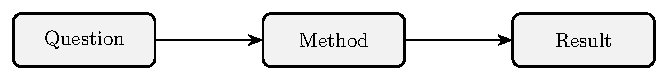
\includegraphics[width=\linewidth]{figures/example-diagram.pdf}
  \end{columns}
\end{frame}

\section{控制变量的理论基础：传统范式}

\begin{frame}{基本的线性结构模型设定}
假设结果变量 $Y_i$ 的真实数据生成过程（data generating process，DGP）是一个线性结构模型：

\begin{equation}
 Y_i = a + bD_i + cX_i + \varepsilon_i, \quad i = 1, \ldots, n.   
 \label{eq:lin_model}
\end{equation}

其中变量分为三类：
\begin{itemize}
  \item $D_i$：研究者感兴趣的处理变量
  \item $X_i$：影响 $Y$ 且与 $D$ 相关的变量（即 $\text{cov}(D_i, X_i) \neq 0$）
  \item $\varepsilon_i$：影响 $Y$ 但与 $D$ 无关的其他因素（即 $\text{cov}(D_i, \varepsilon_i) = 0$）
\end{itemize}
参数 $b$ 就是我们想要估计的因果效应。
\end{frame}

\begin{frame}{ 遗漏变量偏误}
如果研究者不知道或无法观测 $X_i$，只能估计一个简单的一元回归：


\begin{equation}
Y_i = \alpha + \beta D_i + u_i
\end{equation}


用OLS估计 $\beta$，得到的估计量为：

$$
\hat{\beta}^{ols} = \frac{\text{cov}(Y_i, D_i)}{\text{var}(D_i)}.
$$

将真实的DGP代入，可以推导出：

\begin{equation}
\hat{\beta}^{ols} = \frac{\text{cov}(a + bD_i + cX_i + \varepsilon_i,\; D_i)}{\text{var}(D_i)} = b + c \times \underbrace{\frac{\text{cov}(X_i, D_i)}{\text{var}(D_i)}}_{\lambda}
\end{equation}

\end{frame}

\begin{frame}{遗漏变量偏误公式}

\begin{equation*}
\hat{\beta}^{ols} = \frac{\text{cov}(a + bD_i + cX_i + \varepsilon_i,\; D_i)}{\text{var}(D_i)} = b + c \times \underbrace{\frac{\text{cov}(X_i, D_i)}{\text{var}(D_i)}}_{\lambda}
\end{equation*}

\begin{itemize}
  \item $b$ 这就是经典的\textbf{遗漏变量偏误公式}。OLS估计量 $\hat{\beta}^{ols}$ 等于真实因果效应 $b$ 加上一个偏误项 $c \times \lambda$。
  \item 偏误项的含义是：$c$ 是遗漏变量 $X$ 对结果 $Y$ 的影响，$\lambda$ 是遗漏变量 $X$ 与处理变量 $D$ 的关联程度。
  \item 偏误为零需要 $c=0$（$X$ 不影响 $Y$）或 $\lambda=0$（$X$ 与 $D$ 不相关），在观测性研究中这两个条件通常都不满足。
\end{itemize}
\end{frame}


\begin{frame}{ 多元回归与FWL定理}
为了消除偏误，将 $X_i$ 加入回归方程：

\begin{equation}
  Y_i = \alpha^l + \beta^l D_i + \gamma^l X_i + u_i^l
\end{equation}

若满足条件外生性假设 $E[u_i^l \mid D_i, X_i] = 0$，则 $\hat{\beta}^l$ 是因果参数 $b$ 的一致估计。

FWL定理（Frisch -- Waugh -- Lovell Theorem）提供了直观理解：多元回归中 $D_i$ 的系数可以通过两步得到：

\begin{itemize}
  \item 将 $Y_i$ 和 $D_i$ 各自对 $X_i$ 做回归，取残差 $\tilde{Y}_i$ 和 $\tilde{D}_i$，剔除掉能被 $X_i$ 解释的部分。
  \item 将 $\tilde{Y}_i$ 对 $\tilde{D}_i$ 回归，系数 $\hat{\beta}^s = \frac{\text{cov}(\tilde{Y}_i, \tilde{D}_i)}{\text{var}(\tilde{D}_i)}$，与长回归系数完全一致。
  \item 净化后 $\tilde{Y}_i$ 和 $\tilde{D}_i$ 都与 $X_i$ 正交，它们之间的相关性不可能来自遗漏 $X_i$ 导致的伪相关，只能来自 $D_i$ 对 $Y_i$ 的真实因果关系。
\end{itemize}
\end{frame}

\begin{frame}{传统范式面临的挑战}
\begin{itemize}
  \item \textbf{缺乏对因果关系的明确定义}
    \begin{itemize}
      \item 传统方法试图通过结构模型参数定义因果效应，混淆了因果效应、估计目标与估计量。
      \item 结构参数仅为因果效应的函数表示，而非本体。
      \item \textbf{举例：}当存在异质性因果效应（即 $b_i$ 因人而异）时，OLS 估计量 $\hat{\beta}^l$ 的估计目标将变得模糊。
    \end{itemize}
  \vspace{0.5em} % 增加两个主点之间的垂直间距，让排版更透气
  \item \textbf{未区分处理变量和控制变量的角色}
    \begin{itemize}
      \item 处理变量 $D_i$ 和控制变量 $X_i$ 在回归方程中地位对称。
      \item \textbf{逻辑悖论：}基于相关性选择控制变量时，如果说 $X$ 是 $D$ 的遗漏变量，反过来也能成立。
    \end{itemize}
\end{itemize}
\end{frame}
\section{基于设计的研究范式：控制变量的新理解}


\begin{frame}[allowframebreaks]{潜在结果框架(potential outcomes framework)}
\begin{itemize}
  \item 潜在结果 (Potential Outcomes)：对于特定的治疗水平 $w \in \{0, 1\}$，定义潜在结果 $Y_i(1)$ 和 $Y_i(0)$，它们分别代表第 $i$ 个对象在接受治疗或未接受治疗时原本会经历的结果 。实际上观察到的结果 $Y_i$ 取决于该对象最终接受的治疗分配 $W_i$，即 $Y_i = Y_i(W_i)$ 。
  \item 个体因果效应 (Individual Causal Effect)：治疗对第 $i$ 个体的因果效应被定义为其两种潜在结果的差值，接受处理时的 $Y_i(1)$ 和未接受处理时的 $Y_i(0)$。个体因果效应定义为：

\[\tau_i \equiv Y_i(1) - Y_i(0)\]

\item 群体平均因果效应（ATE）为：

\[
ATE \equiv E[\tau_i] = E[Y_i(1) - Y_i(0)]  \not = \underbrace{E[Y|D_i=1] - E[Y|D_i=0]}_{\text{Simple Difference in Means}}
\]

\item 这个定义的优势：不依赖结构模型的函数形式，自然容纳异质性因果效应
\item 因果推断的根本问题 (The Fundamental Problem in Causal Inference)：于任意给定的个体，只能为其分配一种治疗方式，因此 $Y_i(0)$ 和 $Y_i(1)$ 中永远只能观察到其中一个。因果推断本质上是一个\textbf{缺失数据问题}。
\end{itemize}
\end{frame}


\begin{frame}{选择性偏误的来源}
直接比较处理组和对照组的均值差异（Simple Difference in Means，SDM）：

\[
SDM = \underbrace{E[Y_i(1)|D_i=1] - E[Y_i(0)|D_i=1]}_{ATT} + \underbrace{\{E[Y_i(0)|D_i=1] - E[Y_i(0)|D_i=0]\}}_{\text{选择性偏误}}
\]

选择性偏误衡量的是：处理组和对照组即使都不接受处理，其潜在结果也可能不同。

消除选择性偏误需要独立性假设 $\{Y(1), Y(0)\} \perp D$，但在观测性研究中几乎不可能成立。

\vspace{0.5em}

因此，以经济学为代表的使用观测数据开展研究的社会科学领域所面临的因果推断问题，难以直接计算SDM，因为经济学家一般难以开展随机试验。
\end{frame}
\begin{frame}[allowframebreaks]{条件独立性假设与分块随机化实验}

全样本中独立性假设 $\{Y(1), Y(0)\} \perp D$ 几乎不成立，但如果将比较范围缩小到\textbf{特征相同的子样本}中，或许可以在局部实现近似随机。为此引入\textbf{条件独立性假设}（CIA）：
\[
  \{Y(1), Y(0)\} \perp D \mid X
\]
含义：在控制变量 $X$ 取值相同的个体中，处理状态的分配近似于随机。

\vspace{0.8em}

定义\textbf{倾向得分} $e(X) \equiv \Pr\{D=1 \mid X\}$，将 $X$ 取值相同的个体归入同一个\textbf{分块（block）}。CIA 保证分块内部所有个体接受处理的概率相同，此时：
\begin{align*}
  E\big[Y_i(0) \mid D_i=1,\, X\big]
    &= E\big[Y_i(0) \mid D_i=0,\, X\big]
     = E\big[Y_i(0) \mid X\big] \\[0.3em]
  E\big[Y_i(1) \mid D_i=1,\, X\big]
    &= E\big[Y_i(1) \mid D_i=0,\, X\big]
     = E\big[Y_i(1) \mid X\big]
\end{align*}
处理组和对照组在分块内具有相同的潜在结果分布，选择性偏误被消除。于是可以用可观测数据估计分块内的\textbf{条件平均处理效应}：
\[
  \tau(X) = E[Y_i \mid D_i=1,\, X] - E[Y_i \mid D_i=0,\, X]
\]

\framebreak

上述推导还需要一个常被忽略的前提——\textbf{重叠性假设}：
\[
  0 < e(X) < 1 \quad \text{对所有可能的 } X \text{ 取值成立}
\]
它保证每个分块内既有处理组又有对照组。若某分块内 $e(X)=0$ 或 $1$，则找不到比较对象，该分块的因果效应无法识别，相应样本被排除在估计之外。

\vspace{0.8em}

综上，控制变量在分块随机化实验中的操作可归纳为三步：
\begin{enumerate}
  \item \textbf{按控制变量分块}——将 $X$ 取值相同的个体归入同一分块
  \item \textbf{分块内估计条件因果效应}——CIA 保证分块内处理状态近似随机，组间均值差异即为 $\tau(X)$
  \item \textbf{跨组加权平均}——精确匹配估计量：
    \[
      ATE = \sum_{x:\, 0<e_x<1}
        \frac{\Pr(X=x)}{\sum_{x'}\Pr(X=x')} \cdot \tau(X=x)
    \]

\end{enumerate}


  \vspace{1em}
  \begin{quote}
    \Large \textbf{``通过将全样本按照控制变量取值划分为多个分块，在 CIA 假设成立的前提下，每一个分块内部都近似于一个随机化实验。''}
  \end{quote}
  \vspace{1em}

\end{frame}
\section{辛普森悖论（Simpson's Paradox）}

\begin{frame}{Simpson's Paradox: COVID-27}
\href{https://www.youtube.com/playlist?list=PLoazKTcS0RzZ1SUgeOgc6SWt51gfT80N0}{Brady Neal}的slides中用COVID-27的例子说明了Simpson's Paradox。这个例子与\textcite{GLSJ202510012}中"分块随机化实验"的思想在底层原理上完全一致。

\vspace{0.5em}

  \begin{table}
  \centering
  \renewcommand{\arraystretch}{1.3} % 增加行距，防止幻灯片中显得拥挤
  \setlength{\tabcolsep}{10pt}      % 调整列间距
  \begin{tabular}{lccc}
    \toprule
    % 第一列表头跨2行，后面三列的上方加一个跨3列的总表头
    \multirow{2}{*}{\textbf{Treatment}} & \multicolumn{3}{c}{\textbf{Condition}} \\
    \cmidrule(lr){2-4} % 在第2列到第4列下方画一条修饰用的短横线，(lr)表示左右两端稍微缩进
    & \textbf{Mild} & \textbf{Severe} & \textbf{Total} \\
    \midrule
    Treatment A & 210/1400 = 15\% & 30/100 = 30\% & 240/1500 = 16\% \\
    Treatment B & 5/50 = 10\%    & 100/500 = 20\% & 105/550 = 19.1\% \\
    \bottomrule
  \end{tabular}
\end{table}


  朴素比较（不分层）：A的死亡率16\%低于B的19.1\%，A看起来更好。但在每一层内部：轻症中B（10\%）优于A（15\%），重症中B（20\%）优于A（30\%）。这就是Simpson's Paradox——总体趋势与分层趋势方向相反。

\vspace{2em}
\end{frame}

% ============================================================
% Frame 1：问题引入 + Scenario 1（Confounder）
% ============================================================
\begin{frame}{Scenario 1：C 是 Confounder}

  \begin{columns}[c]
    \begin{column}{0.55\textwidth}
      \begin{itemize}
        \item 因果图：$C \to T$，$C \to Y$，$T \to Y$
        \item 病情 $C$ 是\textbf{混杂变量}，同时影响治疗选择和结果
        \item \textbf{应该控制} $C$
      \end{itemize}

      \medskip

      \begin{exampleblock}{直觉}
        新冠疫情中，轻症患者进方舱接受传统医学干预，重症患者进ICU接受现代医学干预。病情严重程度同时决定了治疗分配和死亡率，直接对比两种处理有失公允。
      \end{exampleblock}
    \end{column}

    \begin{column}{0.4\textwidth}
      \centering
      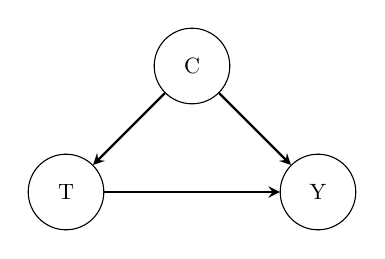
\begin{tikzpicture}[scale=0.8, every node/.style={scale=0.8}]
        \tikzstyle{circ} = [draw, circle, minimum size=1.2cm, align=center, inner sep=1pt]
        \node[circ] (T) at (0, 0) {T};
        \node[circ] (Y) at (4, 0) {Y};
        \node[circ] (C) at (2, 2) {C};
        \draw[->, >=stealth, thick] (C) -- (T);
        \draw[->, >=stealth, thick] (C) -- (Y);
        \draw[->, >=stealth, thick] (T) -- (Y);
      \end{tikzpicture}
    \end{column}
  \end{columns}

\end{frame}

% ============================================================
% Frame 2：Scenario 2（Mediator）
% ============================================================
\begin{frame}{Scenario 2：C 是 Mediator}

  \begin{columns}[c]
    \begin{column}{0.55\textwidth}
      \begin{itemize}
        \item 因果图：$T \to C \to Y$，$T \to Y$
        \item 治疗 $T$ 影响病情 $C$（如副作用导致病情加重），$C$ 是\textbf{中介变量}
        \item \textbf{不应该控制} $C$
      \end{itemize}

      \medskip

      \begin{exampleblock}{直觉}
        如果 Treatment B 需要患者等待很长时间，等待本身导致病情加重，那么"病情加重"是治疗的后果，不是预先存在的混杂。在回归中控制它会遮蔽治疗的真实总效应。
      \end{exampleblock}
    \end{column}

    \begin{column}{0.4\textwidth}
      \centering
      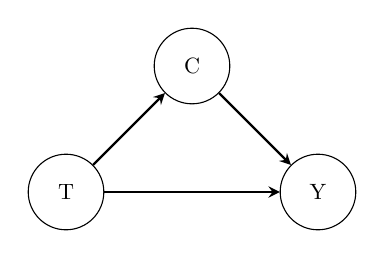
\begin{tikzpicture}[scale=0.8, every node/.style={scale=0.8}]
        \tikzstyle{circ} = [draw, circle, minimum size=1.2cm, align=center, inner sep=1pt]
        \node[circ] (T) at (0, 0) {T};
        \node[circ] (Y) at (4, 0) {Y};
        \node[circ] (C) at (2, 2) {C};
        \draw[->, >=stealth, thick] (T) -- (C);
        \draw[->, >=stealth, thick] (C) -- (Y);
        \draw[->, >=stealth, thick] (T) -- (Y);
      \end{tikzpicture}
    \end{column}
  \end{columns}

\end{frame}

% ============================================================
% Frame 3：对比表格 + 效应分解 + 核心启示
% ============================================================
\begin{frame}[allowframebreaks]{同样的数据，完全相反的结论}

  \begin{table}
  \centering
  \begin{tabular}{l|c|c}
    \hline
     & \textbf{Scenario 1 (Confounder)} & \textbf{Scenario 2 (Mediator)} \\
    \hline
    因果图 & $C \to T$，$C \to Y$，$T \to Y$ & $T \to C \to Y$，$T \to Y$ \\
    观测数据 & 完全相同 & 完全相同 \\
    应该控制C吗 & \checkmark{} 应该 & $\times$ 不应该 \\
    \texttt{reg Y T} 的系数 & +0.031（$\times$ 有偏） & +0.031（\checkmark{} 无偏） \\
    \texttt{reg Y T C} 的系数 & $-$0.082（\checkmark{} 无偏） & $-$0.082（$\times$ 有偏） \\
    正确的因果效应 & $-$0.065 & +0.031 \\
    应该选择 & \textbf{Treatment B} & \textbf{Treatment A} \\
    \hline
  \end{tabular}
  \caption{两个Scenario的结果对比}
  \end{table}

  \begin{block}{效应分解（Scenario 2）}
    Treatment B 的总效应可分解为：

    $$\underbrace{+0.031}_{\text{总效应}} = \underbrace{-0.082}_{\text{直接效应}} + \underbrace{+0.113}_{\text{间接效应}}$$

    B 的直接治疗效果更好，但副作用让病情加重（间接效应为正），导致总效应反而增加死亡率。
  \end{block}

  \begin{alertblock}{核心启示}
    同样的数据 $+$ 不同的因果结构 $=$ 完全相反的结论。

    \medskip

    如果错误地控制了中介变量 $C$，只能看到直接效应 $-0.082$，从而错误地选择 B。

    \medskip

    这完美对应了\parencite{GLSJ202510012}的原则一：\textbf{控制变量的选择必须基于因果结构，而非数据本身。}
  \end{alertblock}

\end{frame}

% ============================================================
% Frame 4：后门调整公式（以 Scenario 1 为例）
% ============================================================
\begin{frame}[allowframebreaks]{后门调整公式：怎样正确控制 Confounder？}

  \begin{block}{核心思想}
    既然 Scenario 1 中应该控制 $C$，具体怎么做？——后门调整公式：
    $$E[Y \mid do(T=t)] = \sum_c E[Y \mid t, c] \cdot P(c)$$
  \end{block}

  \begin{block}{操作步骤}
    \begin{enumerate}
      \item \textbf{分层：} 按 $C$ 的取值分为 Mild 和 Severe 两组
      \item \textbf{组内比较：} 每组内部估计条件因果效应（$\tau_{\text{Mild}}=-5\%$，$\tau_{\text{Severe}}=-10\%$）
      \item \textbf{加权平均：} 用总体中各层比例加权（$P(\text{Mild})=\frac{1450}{2050}$，$P(\text{Severe})=\frac{600}{2050}$）
    \end{enumerate}
  \end{block}

  \begin{exampleblock}{计算结果}
    \begin{align*}
      E[Y|do(T=A)] &= 0.15 \times \tfrac{1450}{2050} + 0.30 \times \tfrac{600}{2050} = 19.4\% \\
      E[Y|do(T=B)] &= 0.10 \times \tfrac{1450}{2050} + 0.20 \times \tfrac{600}{2050} = 12.9\%
    \end{align*}
    \textbf{结论：} B 的因果死亡率（12.9\%）低于 A（19.4\%），\textbf{应该选 B}。
  \end{exampleblock}

\end{frame}


% ============================================================
% Frame: 线性回归与饱和回归的关系
% ============================================================
\begin{frame}[allowframebreaks]{线性回归与饱和回归的关系}

  \begin{block}{两者的区别}
    当控制变量是离散的且取值不多时：
    \begin{itemize}
      \item \textbf{饱和回归：} 对每个取值放一个虚拟变量，不施加任何函数形式限制
      \item \textbf{线性回归：} 把控制变量当作连续变量，隐含了线性假设
    \end{itemize}
  \end{block}

  \begin{block}{精确数学关系（张文公式20）}
    $$\beta^{ols} = \beta^{sat} + \frac{\text{var}(e(X_i) - L(X_i))}{\text{var}(D_i - L(X_i))} \left[\beta^{sat} - \frac{\text{cov}[(e(X_i) - L(X_i))Y_i]}{\text{var}(e(X_i) - L(X_i))}\right]$$

    \medskip
    \footnotesize
    $e(X_i)$：真实倾向得分（饱和回归隐含估计）；$L(X_i)$：线性回归用线性概率模型估计的倾向得分。

    \medskip
    \normalsize
    \textbf{核心信息：} 当 $e(X_i) = L(X_i)$ 时，第二项为零，两者完全一致。即倾向得分恰好是控制变量的线性函数时，两种回归给出相同结果。
  \end{block}

  \begin{exampleblock}{COVID-27 中为什么两者相等？}
    控制变量 $C$ 只有两个取值（0和1）。对二值变量而言，任何函数都可以用线性函数精确表示——两个点总能被一条直线完美连接。

    \medskip

    所以 $e(X) = L(X)$，线性回归和饱和回归的系数完全一致。
  \end{exampleblock}

  \begin{alertblock}{什么时候两者会不同？}
    如果控制变量有三个或更多取值，且倾向得分与控制变量的关系不是线性的，两者就会产生差异。

    \medskip

    例如病情分为轻/中/重三类，倾向得分分别是 $0.03$、$0.50$、$0.90$。线性回归强制拟合一条直线，但中间值 $0.50$ 偏离了轻和重的连线中点 $0.465$，导致 $L(X) \neq e(X)$。

    \medskip

    这就是\parencite{GLSJ202510012}所说的\textbf{模型误设偏误}（misspecification bias）——线性回归对倾向得分做了错误的线性假设，导致匹配不准确。
  \end{alertblock}

  \begin{block}{一句话总结}
    饱和回归是``无约束版''的分块比较，线性回归是``线性约束版''的分块比较。
    \medskip

    两者的研究设计完全相同（按控制变量分块、组内比较、加权平均），区别仅在于线性回归额外假设了倾向得分是控制变量的线性函数。

    \medskip
    当假设成立时两者等价，不成立时线性回归会有\textbf{外推偏误}。
  \end{block}
\end{frame}
\section{结论}
% ============================================================
% Frame: 好控制变量
% ============================================================
\begin{frame}[allowframebreaks]{好控制变量}

  % --- 好控制变量1: 共同原因X ---
  \begin{columns}[c]
    \begin{column}{0.55\textwidth}
      \begin{block}{1. D和Y的共同原因X}
        X同时影响D和Y，不控制会导致遗漏变量偏误。控制X后，分块内部处理状态近似随机，选择性偏误被消除。

        \medskip
        \textbf{应该控制。}
      \end{block}
    \end{column}
    \begin{column}{0.4\textwidth}
      \centering
      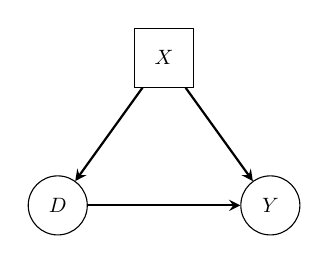
\begin{tikzpicture}[scale=0.75, every node/.style={scale=0.75}]
        \tikzstyle{circ} = [draw, circle, minimum size=1cm, align=center, inner sep=1pt]
        \tikzstyle{sq} = [draw, rectangle, minimum size=1cm, align=center, inner sep=1pt]
        \node[sq] (X) at (1, 2.5) {$X$};
        \node[circ] (D) at (-0.8, 0) {$D$};
        \node[circ] (Y) at (2.8, 0) {$Y$};
        \draw[->, >=stealth, thick] (X) -- (D);
        \draw[->, >=stealth, thick] (X) -- (Y);
        \draw[->, >=stealth, thick] (D) -- (Y);
      \end{tikzpicture}

      {\footnotesize \fbox{方框} $=$ 好控制变量}
    \end{column}
  \end{columns}

  \framebreak

  % --- 好控制变量2: 代理变量G ---
  \begin{columns}[c]
    \begin{column}{0.55\textwidth}
      \begin{block}{2. 遗漏变量$\varepsilon$的代理变量G}
        如果$\varepsilon$无法直接观测，但G是$\varepsilon$影响D的机制变量（$\varepsilon \to G \to D$），控制G可间接剥离D和$\varepsilon$的相关性。

        \medskip
        \textbf{应该控制。}
      \end{block}
    \end{column}
    \begin{column}{0.4\textwidth}
      \centering
      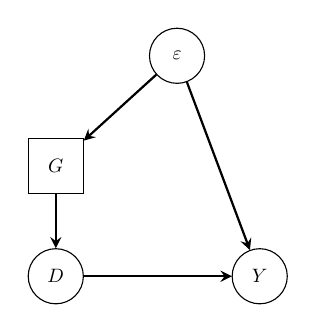
\begin{tikzpicture}[scale=0.7, every node/.style={scale=0.7}]
        \tikzstyle{circ} = [draw, circle, minimum size=1cm, align=center, inner sep=1pt]
        \tikzstyle{sq} = [draw, rectangle, minimum size=1cm, align=center, inner sep=1pt]
        \node[circ] (eps) at (1, 4) {$\varepsilon$};
        \node[sq] (G) at (-1.2, 2) {$G$};
        \node[circ] (D) at (-1.2, 0) {$D$};
        \node[circ] (Y) at (2.5, 0) {$Y$};
        \draw[->, >=stealth, thick] (eps) -- (G);
        \draw[->, >=stealth, thick] (eps) -- (Y);
        \draw[->, >=stealth, thick] (G) -- (D);
        \draw[->, >=stealth, thick] (D) -- (Y);
      \end{tikzpicture}
    \end{column}
  \end{columns}

  \framebreak

  % --- 好控制变量3: Y的原因P ---
  \begin{columns}[c]
    \begin{column}{0.55\textwidth}
      \begin{block}{3. Y的原因变量P，且与D无关}
        控制P能吸收误差项方差，降低标准误，提高统计功效。因P与D无关，不会吸收处理变量的变异性。

        \medskip
        纯粹提高精度，不影响因果识别。
      \end{block}
    \end{column}
    \begin{column}{0.4\textwidth}
      \centering
      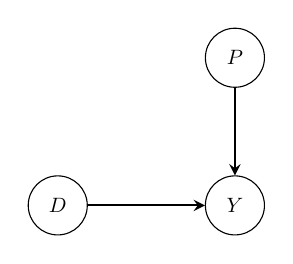
\begin{tikzpicture}[scale=0.75, every node/.style={scale=0.75}]
        \tikzstyle{circ} = [draw, circle, minimum size=1cm, align=center, inner sep=1pt]
        \node[circ] (D) at (-1, 0) {$D$};
        \node[circ] (Y) at (2, 0) {$Y$};
        \node[circ] (P) at (2, 2.5) {$P$};
        \draw[->, >=stealth, thick] (D) -- (Y);
        \draw[->, >=stealth, thick] (P) -- (Y);
      \end{tikzpicture}
    \end{column}
  \end{columns}

\end{frame}

% ============================================================
% Frame: 坏控制变量
% ============================================================
\begin{frame}[allowframebreaks]{坏控制变量}

  % --- 坏控制变量1: 对撞变量Q ---
  \begin{columns}[c]
    \begin{column}{0.55\textwidth}
      \begin{alertblock}{1. 对撞变量（Collider）Q}
        Q是D和u（影响Y的因素）的共同结果。不控制时D和u不相关；控制Q后，D和u人为产生相关性，凭空引入选择性偏误。

        \medskip
        \textbf{不应该控制。}
      \end{alertblock}
    \end{column}
    \begin{column}{0.4\textwidth}
      \centering
      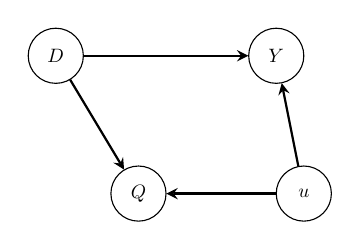
\begin{tikzpicture}[scale=0.7, every node/.style={scale=0.7}]
        \tikzstyle{circ} = [draw, circle, minimum size=1cm, align=center, inner sep=1pt]
        \node[circ] (D) at (-1.5, 2.5) {$D$};
        \node[circ] (Y) at (2.5, 2.5) {$Y$};
        \node[circ] (Q) at (0, 0) {$Q$};
        \node[circ] (u) at (3, 0) {$u$};
        \draw[->, >=stealth, thick] (D) -- (Y);
        \draw[->, >=stealth, thick] (D) -- (Q);
        \draw[->, >=stealth, thick] (u) -- (Q);
        \draw[->, >=stealth, thick] (u) -- (Y);
      \end{tikzpicture}

      {\footnotesize 圆圈 $=$ 坏控制变量}
    \end{column}
  \end{columns}

  \framebreak

  % --- 坏控制变量2a: 中介变量M（简单情形）---
  \begin{columns}[c]
    \begin{column}{0.55\textwidth}
      \begin{alertblock}{2a. 中介变量（Mediator）W}
        $D \to W \to Y$ 路径上的变量。控制W会阻断间接效应路径，只剩直接效应，低估甚至反转总因果效应的方向。

        \medskip
        \textbf{不应该控制——过度控制。}
      \end{alertblock}
    \end{column}
    \begin{column}{0.4\textwidth}
      \centering
      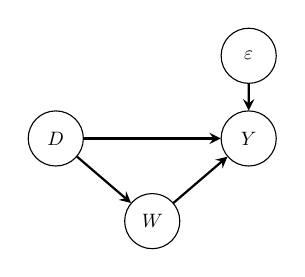
\begin{tikzpicture}[scale=0.7, every node/.style={scale=0.7}]
        \tikzstyle{circ} = [draw, circle, minimum size=1cm, align=center, inner sep=1pt]
        \node[circ] (eps) at (2.5, 3) {$\varepsilon$};
        \node[circ] (D) at (-1, 1.5) {$D$};
        \node[circ] (Y) at (2.5, 1.5) {$Y$};
        \node[circ] (W) at (0.75, 0) {$W$};
        \draw[->, >=stealth, thick] (D) -- (Y);
        \draw[->, >=stealth, thick] (D) -- (W);
        \draw[->, >=stealth, thick] (W) -- (Y);
        \draw[->, >=stealth, thick] (eps) -- (Y);
      \end{tikzpicture}
    \end{column}
  \end{columns}

  \framebreak

  % --- 坏控制变量2b: 中介 + 对撞（复合情形）---
  \begin{columns}[c]
    \begin{column}{0.55\textwidth}
      \begin{alertblock}{2b. 中介变量同时也是对撞变量}
        现实中几乎一定存在不可观测因素u同时影响W和Y。此时W同时是中介和对撞变量，控制它会同时产生过度控制和对撞偏误。

        \medskip
        \textbf{双重危害。}
      \end{alertblock}
    \end{column}
    \begin{column}{0.4\textwidth}
      \centering
    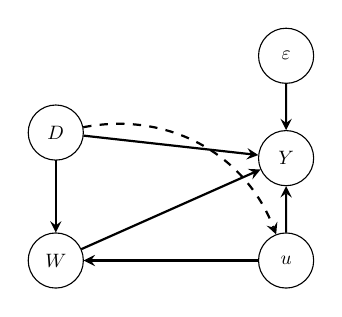
\begin{tikzpicture}[scale=0.65, every node/.style={scale=0.7}]
  \tikzstyle{circ} = [draw, circle, minimum size=1cm, align=center, inner sep=1pt]
  \node[circ] (eps) at (3, 3.5) {$\varepsilon$};
  \node[circ] (D) at (-1.5, 2) {$D$};
  \node[circ] (Y) at (3, 1.5) {$Y$};
  \node[circ] (W) at (-1.5, -0.5) {$W$};
  \node[circ] (u) at (3, -0.5) {$u$};
  \draw[->, >=stealth, thick] (D) -- (Y);
  \draw[->, >=stealth, thick] (D) -- (W);
  \draw[->, >=stealth, thick] (W) -- (Y);
  \draw[->, >=stealth, thick] (u) -- (W);
  \draw[->, >=stealth, thick] (u) -- (Y);
  \draw[->, >=stealth, thick] (eps) -- (Y);
  \draw[->, >=stealth, thick, dashed] (D) to[bend left=40] (u);
\end{tikzpicture}
    \end{column}
  \end{columns}

  \framebreak

  % --- 坏控制变量3: Y的结果变量R ---
  \begin{columns}[c]
    \begin{column}{0.55\textwidth}
      \begin{alertblock}{3. Y的结果变量R}
        控制R会将潜在结果不可比的群体放在一起比较，产生选择性偏误。

        \medskip
        \textbf{不应该控制。}
      \end{alertblock}
    \end{column}
    \begin{column}{0.4\textwidth}
      \centering
      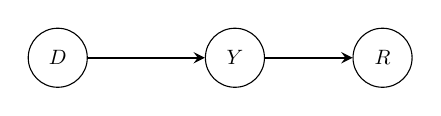
\begin{tikzpicture}[scale=0.75, every node/.style={scale=0.75}]
        \tikzstyle{circ} = [draw, circle, minimum size=1cm, align=center, inner sep=1pt]
        \node[circ] (D) at (-1.5, 0) {$D$};
        \node[circ] (Y) at (1.5, 0) {$Y$};
        \node[circ] (R) at (4, 0) {$R$};
        \draw[->, >=stealth, thick] (D) -- (Y);
        \draw[->, >=stealth, thick] (Y) -- (R);
      \end{tikzpicture}
    \end{column}
  \end{columns}

  \framebreak

  % --- 坏控制变量4: D的原因W ---
\begin{columns}[c]
    \begin{column}{0.55\textwidth}
      \begin{alertblock}{4. D的原因变量W（统计推断层面）}
        控制W会大量吸收处理变量D的变异性，导致标准误显著增大、统计功效下降。虽不引入偏误，但让估计变得非常不精确。

        \medskip
        \textbf{不建议控制。}
      \end{alertblock}
    \end{column}
    \begin{column}{0.4\textwidth}
      \centering
    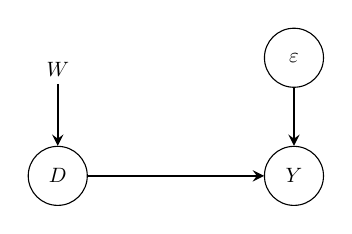
\begin{tikzpicture}[scale=0.75, every node/.style={scale=0.75}]
  \tikzstyle{circ} = [draw, circle, minimum size=1cm, align=center, inner sep=1pt]
  \node[circ] (eps) at (2.5, 2) {$\varepsilon$};
  \node (W) at (-1.5, 1.8) {$W$};
  \node[circ] (D) at (-1.5, 0) {$D$};
  \node[circ] (Y) at (2.5, 0) {$Y$};
  \draw[->, >=stealth, thick] (W) -- (D);
  \draw[->, >=stealth, thick] (D) -- (Y);
  \draw[->, >=stealth, thick] (eps) -- (Y);
\end{tikzpicture}
    \end{column}
  \end{columns}

\end{frame}

% ============================================================
% Frame: 总览图
% ============================================================

\begin{frame}{控制变量分类总览}

  \begin{center}
  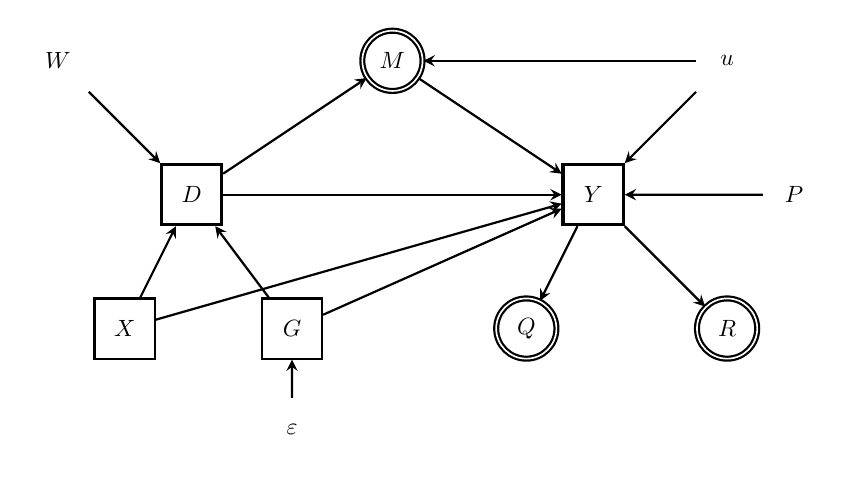
\begin{tikzpicture}[scale=0.85, every node/.style={scale=0.85},
    >=stealth, thick,
    good/.style={draw, rectangle, minimum size=0.9cm, align=center, inner sep=3pt},
    bad/.style={draw, circle, minimum size=0.9cm, align=center, double},
    core/.style={draw, rectangle, minimum size=0.9cm, align=center, inner sep=3pt, line width=1.2pt},
    plain/.style={minimum size=0.9cm, align=center}]

    % === 第一行: W, M, u, P (y=4) ===
    \node[plain] (W) at (-5, 4) {$W$};
    \node[bad]   (M) at (0, 4)  {$M$};
    \node[plain] (u) at (5, 4)  {$u$};

    % === 第二行: D, Y, P (y=2) ===
    \node[core]  (D) at (-3, 2) {$D$};
    \node[core]  (Y) at (3, 2)  {$Y$};
    \node[plain] (P) at (6, 2)  {$P$};

    % === 第三行: X, G, Q, R (y=0) ===
    \node[good]  (X) at (-4, 0) {$X$};
    \node[good]  (G) at (-1.5, 0) {$G$};
    \node[bad]   (Q) at (2, 0)  {$Q$};
    \node[bad]   (R) at (5, 0)  {$R$};

    % === 第四行: epsilon (y=-1.5) ===
    \node[plain] (eps) at (-1.5, -1.5) {$\varepsilon$};

    % === 连线 ===
    % W → D
    \draw[->] (W) -- (D);

    % D → Y (核心因果路径)
    \draw[->] (D) -- (Y);

    % D → M, M → Y (中介路径)
    \draw[->] (D) -- (M);
    \draw[->] (M) -- (Y);

    % u → M, u → Y
    \draw[->] (u) -- (M);
    \draw[->] (u) -- (Y);

    % P → Y
    \draw[->] (P) -- (Y);

    % Y → Q, Y → R
    \draw[->] (Y) -- (Q);
    \draw[->] (Y) -- (R);

    % X → D, X → Y
    \draw[->] (X) -- (D);
    \draw[->] (X) -- (Y);

    % G → D, G → Y
    \draw[->] (G) -- (D);
    \draw[->] (G) -- (Y);

    % eps → G
    \draw[->] (eps) -- (G);

  \end{tikzpicture}
  \end{center}

  \vspace{0.3em}
  \centering
  \footnotesize
  \fbox{方框} $=$ 因果识别的好控制变量 \qquad
  \tikz\draw[double, thick] (0,0) circle (0.3cm); $=$ 坏控制变量

\end{frame}

\begin{frame}{References}
  \printbibliography
\end{frame}

\end{document}
